% Options for packages loaded elsewhere
\PassOptionsToPackage{unicode}{hyperref}
\PassOptionsToPackage{hyphens}{url}
%
\documentclass[
]{book}
\usepackage{amsmath,amssymb}
\usepackage{lmodern}
\usepackage{ifxetex,ifluatex}
\ifnum 0\ifxetex 1\fi\ifluatex 1\fi=0 % if pdftex
  \usepackage[T1]{fontenc}
  \usepackage[utf8]{inputenc}
  \usepackage{textcomp} % provide euro and other symbols
\else % if luatex or xetex
  \usepackage{unicode-math}
  \defaultfontfeatures{Scale=MatchLowercase}
  \defaultfontfeatures[\rmfamily]{Ligatures=TeX,Scale=1}
\fi
% Use upquote if available, for straight quotes in verbatim environments
\IfFileExists{upquote.sty}{\usepackage{upquote}}{}
\IfFileExists{microtype.sty}{% use microtype if available
  \usepackage[]{microtype}
  \UseMicrotypeSet[protrusion]{basicmath} % disable protrusion for tt fonts
}{}
\makeatletter
\@ifundefined{KOMAClassName}{% if non-KOMA class
  \IfFileExists{parskip.sty}{%
    \usepackage{parskip}
  }{% else
    \setlength{\parindent}{0pt}
    \setlength{\parskip}{6pt plus 2pt minus 1pt}}
}{% if KOMA class
  \KOMAoptions{parskip=half}}
\makeatother
\usepackage{xcolor}
\IfFileExists{xurl.sty}{\usepackage{xurl}}{} % add URL line breaks if available
\IfFileExists{bookmark.sty}{\usepackage{bookmark}}{\usepackage{hyperref}}
\hypersetup{
  pdftitle={A GitBook template},
  pdfauthor={Nikola Sekulovski},
  hidelinks,
  pdfcreator={LaTeX via pandoc}}
\urlstyle{same} % disable monospaced font for URLs
\usepackage{color}
\usepackage{fancyvrb}
\newcommand{\VerbBar}{|}
\newcommand{\VERB}{\Verb[commandchars=\\\{\}]}
\DefineVerbatimEnvironment{Highlighting}{Verbatim}{commandchars=\\\{\}}
% Add ',fontsize=\small' for more characters per line
\usepackage{framed}
\definecolor{shadecolor}{RGB}{248,248,248}
\newenvironment{Shaded}{\begin{snugshade}}{\end{snugshade}}
\newcommand{\AlertTok}[1]{\textcolor[rgb]{0.94,0.16,0.16}{#1}}
\newcommand{\AnnotationTok}[1]{\textcolor[rgb]{0.56,0.35,0.01}{\textbf{\textit{#1}}}}
\newcommand{\AttributeTok}[1]{\textcolor[rgb]{0.77,0.63,0.00}{#1}}
\newcommand{\BaseNTok}[1]{\textcolor[rgb]{0.00,0.00,0.81}{#1}}
\newcommand{\BuiltInTok}[1]{#1}
\newcommand{\CharTok}[1]{\textcolor[rgb]{0.31,0.60,0.02}{#1}}
\newcommand{\CommentTok}[1]{\textcolor[rgb]{0.56,0.35,0.01}{\textit{#1}}}
\newcommand{\CommentVarTok}[1]{\textcolor[rgb]{0.56,0.35,0.01}{\textbf{\textit{#1}}}}
\newcommand{\ConstantTok}[1]{\textcolor[rgb]{0.00,0.00,0.00}{#1}}
\newcommand{\ControlFlowTok}[1]{\textcolor[rgb]{0.13,0.29,0.53}{\textbf{#1}}}
\newcommand{\DataTypeTok}[1]{\textcolor[rgb]{0.13,0.29,0.53}{#1}}
\newcommand{\DecValTok}[1]{\textcolor[rgb]{0.00,0.00,0.81}{#1}}
\newcommand{\DocumentationTok}[1]{\textcolor[rgb]{0.56,0.35,0.01}{\textbf{\textit{#1}}}}
\newcommand{\ErrorTok}[1]{\textcolor[rgb]{0.64,0.00,0.00}{\textbf{#1}}}
\newcommand{\ExtensionTok}[1]{#1}
\newcommand{\FloatTok}[1]{\textcolor[rgb]{0.00,0.00,0.81}{#1}}
\newcommand{\FunctionTok}[1]{\textcolor[rgb]{0.00,0.00,0.00}{#1}}
\newcommand{\ImportTok}[1]{#1}
\newcommand{\InformationTok}[1]{\textcolor[rgb]{0.56,0.35,0.01}{\textbf{\textit{#1}}}}
\newcommand{\KeywordTok}[1]{\textcolor[rgb]{0.13,0.29,0.53}{\textbf{#1}}}
\newcommand{\NormalTok}[1]{#1}
\newcommand{\OperatorTok}[1]{\textcolor[rgb]{0.81,0.36,0.00}{\textbf{#1}}}
\newcommand{\OtherTok}[1]{\textcolor[rgb]{0.56,0.35,0.01}{#1}}
\newcommand{\PreprocessorTok}[1]{\textcolor[rgb]{0.56,0.35,0.01}{\textit{#1}}}
\newcommand{\RegionMarkerTok}[1]{#1}
\newcommand{\SpecialCharTok}[1]{\textcolor[rgb]{0.00,0.00,0.00}{#1}}
\newcommand{\SpecialStringTok}[1]{\textcolor[rgb]{0.31,0.60,0.02}{#1}}
\newcommand{\StringTok}[1]{\textcolor[rgb]{0.31,0.60,0.02}{#1}}
\newcommand{\VariableTok}[1]{\textcolor[rgb]{0.00,0.00,0.00}{#1}}
\newcommand{\VerbatimStringTok}[1]{\textcolor[rgb]{0.31,0.60,0.02}{#1}}
\newcommand{\WarningTok}[1]{\textcolor[rgb]{0.56,0.35,0.01}{\textbf{\textit{#1}}}}
\usepackage{longtable,booktabs,array}
\usepackage{calc} % for calculating minipage widths
% Correct order of tables after \paragraph or \subparagraph
\usepackage{etoolbox}
\makeatletter
\patchcmd\longtable{\par}{\if@noskipsec\mbox{}\fi\par}{}{}
\makeatother
% Allow footnotes in longtable head/foot
\IfFileExists{footnotehyper.sty}{\usepackage{footnotehyper}}{\usepackage{footnote}}
\makesavenoteenv{longtable}
\usepackage{graphicx}
\makeatletter
\def\maxwidth{\ifdim\Gin@nat@width>\linewidth\linewidth\else\Gin@nat@width\fi}
\def\maxheight{\ifdim\Gin@nat@height>\textheight\textheight\else\Gin@nat@height\fi}
\makeatother
% Scale images if necessary, so that they will not overflow the page
% margins by default, and it is still possible to overwrite the defaults
% using explicit options in \includegraphics[width, height, ...]{}
\setkeys{Gin}{width=\maxwidth,height=\maxheight,keepaspectratio}
% Set default figure placement to htbp
\makeatletter
\def\fps@figure{htbp}
\makeatother
\setlength{\emergencystretch}{3em} % prevent overfull lines
\providecommand{\tightlist}{%
  \setlength{\itemsep}{0pt}\setlength{\parskip}{0pt}}
\setcounter{secnumdepth}{5}
\usepackage{booktabs}
\usepackage{amsthm}
\makeatletter
\def\thm@space@setup{%
  \thm@preskip=8pt plus 2pt minus 4pt
  \thm@postskip=\thm@preskip
}
\makeatother
\usepackage{booktabs}
\usepackage{longtable}
\usepackage{array}
\usepackage{multirow}
\usepackage{wrapfig}
\usepackage{float}
\usepackage{colortbl}
\usepackage{pdflscape}
\usepackage{tabu}
\usepackage{threeparttable}
\usepackage{threeparttablex}
\usepackage[normalem]{ulem}
\usepackage{makecell}
\usepackage{xcolor}
\ifluatex
  \usepackage{selnolig}  % disable illegal ligatures
\fi
\usepackage[]{natbib}
\bibliographystyle{apalike}

\title{A GitBook template}
\author{Nikola Sekulovski}
\date{2021-09-29}

\begin{document}
\maketitle

{
\setcounter{tocdepth}{1}
\tableofcontents
}
\hypertarget{introduction}{%
\chapter{Introduction}\label{introduction}}

This is a template GitBook based on \href{https://cjvanlissa.github.io/gitbook-demo/}{\emph{A GitBook Example for Teaching}} and \href{https://bookdown.org/yihui/bookdown/}{\emph{bookdown: Authoring Books and Technical Documents with R Markdown}}.

\hypertarget{monte-carlo-simulations}{%
\chapter{Monte Carlo Simulations}\label{monte-carlo-simulations}}

\begin{Shaded}
\begin{Highlighting}[]
\FunctionTok{library}\NormalTok{(tidyverse)}
\end{Highlighting}
\end{Shaded}

\hypertarget{the-confidence-interval}{%
\section{The Confidence Interval}\label{the-confidence-interval}}

In this exercise I will try to repeat the example given by \href{https://www.gerkovink.com/markup/Wk1/Solution_to_Ex1.html}{Gerko Vink}

The main idea of this exercise is to illustrate the nature of the \emph{Confidence Interval} as described by \href{http://www.stat.cmu.edu/~brian/905-2008/papers/neyman-1934-jrss.pdf}{Neyman (1934)}

We set a seed to make our results reproducible:

\begin{Shaded}
\begin{Highlighting}[]
\FunctionTok{set.seed}\NormalTok{(}\DecValTok{6465}\NormalTok{)}
\end{Highlighting}
\end{Shaded}

\begin{itemize}
\tightlist
\item
  The first step is to take 100 samples (in this case of size 800) from a \emph{normal distributuon} with \(\mu = 0\) and \(\sigma = 1\):
\end{itemize}

\begin{Shaded}
\begin{Highlighting}[]
\NormalTok{samples }\OtherTok{\textless{}{-}}\NormalTok{plyr}\SpecialCharTok{::}\FunctionTok{rlply}\NormalTok{(}\DecValTok{100}\NormalTok{, }\FunctionTok{rnorm}\NormalTok{(}\DecValTok{800}\NormalTok{, }\DecValTok{0}\NormalTok{, }\DecValTok{1}\NormalTok{))}
\end{Highlighting}
\end{Shaded}

\begin{itemize}
\tightlist
\item
  Secondly, we need to calculate for the mean of each sample: the absolute bias; standard error lower bound of the 95\% confidence interval and upper bound of the 95\% confidence interval.
\end{itemize}

We can construct a function that does this:

\begin{Shaded}
\begin{Highlighting}[]
\NormalTok{samp\_function }\OtherTok{\textless{}{-}} \ControlFlowTok{function}\NormalTok{(x) \{}
 
\NormalTok{  m }\OtherTok{\textless{}{-}} \FunctionTok{mean}\NormalTok{(x)}
\NormalTok{  n }\OtherTok{\textless{}{-}} \FunctionTok{length}\NormalTok{(x)}
\NormalTok{  se }\OtherTok{\textless{}{-}} \DecValTok{1}\SpecialCharTok{/}\FunctionTok{sqrt}\NormalTok{(n)}
\NormalTok{  bias }\OtherTok{\textless{}{-}} \FunctionTok{abs}\NormalTok{(}\SpecialCharTok{{-}}\DecValTok{0} \SpecialCharTok{{-}}\NormalTok{ m)}
\NormalTok{  df }\OtherTok{\textless{}{-}}\NormalTok{ n }\SpecialCharTok{{-}} \DecValTok{1}
\NormalTok{  interval }\OtherTok{\textless{}{-}} \FunctionTok{qt}\NormalTok{(.}\DecValTok{975}\NormalTok{, df) }\SpecialCharTok{*}\NormalTok{ se}
  \FunctionTok{return}\NormalTok{(}\FunctionTok{c}\NormalTok{(m, bias, se, m }\SpecialCharTok{{-}}\NormalTok{ interval, m }\SpecialCharTok{+}\NormalTok{ interval))}

\NormalTok{\}}

\NormalTok{format }\OtherTok{\textless{}{-}} \FunctionTok{c}\NormalTok{(}\StringTok{"Mean"} \OtherTok{=} \DecValTok{0}\NormalTok{, }\StringTok{"Bias"} \OtherTok{=} \DecValTok{0}\NormalTok{, }\StringTok{"Std.Err"} \OtherTok{=} \DecValTok{0}\NormalTok{, }\StringTok{"Lower"} \OtherTok{=} \DecValTok{0}\NormalTok{, }\StringTok{"Upper"} \OtherTok{=} \DecValTok{0}\NormalTok{)}
\end{Highlighting}
\end{Shaded}

Now we use the constructed function \texttt{samp\_function} on all 100 samples contained in the object \texttt{samples}. And we also add a new column to the results that indicates which CI of the respective samples does contain \(\mu\).

\begin{Shaded}
\begin{Highlighting}[]
\NormalTok{results }\OtherTok{\textless{}{-}}\NormalTok{ samples }\SpecialCharTok{\%\textgreater{}\%}
  \FunctionTok{vapply}\NormalTok{(., samp\_function, format) }\SpecialCharTok{\%\textgreater{}\%}
\NormalTok{  t }\SpecialCharTok{\%\textgreater{}\%}
\NormalTok{  as\_tibble }\SpecialCharTok{\%\textgreater{}\%} 
  \FunctionTok{mutate}\NormalTok{(}\AttributeTok{Covered =} \FunctionTok{ifelse}\NormalTok{(Lower }\SpecialCharTok{\textless{}} \DecValTok{0} \SpecialCharTok{\&}\NormalTok{ Upper }\SpecialCharTok{\textgreater{}} \DecValTok{0}\NormalTok{, }\DecValTok{1}\NormalTok{, }\DecValTok{0}\NormalTok{))}
\end{Highlighting}
\end{Shaded}

We can also add a table with the sample statistics of the samples whose CI's do not contain \(\mu\).

\begin{Shaded}
\begin{Highlighting}[]
\NormalTok{results }\SpecialCharTok{\%\textgreater{}\%}
  \FunctionTok{filter}\NormalTok{(Covered }\SpecialCharTok{==}\DecValTok{0}\NormalTok{) }\SpecialCharTok{\%\textgreater{}\%}
\NormalTok{  kableExtra}\SpecialCharTok{::}\FunctionTok{kable}\NormalTok{(}\AttributeTok{caption =} \StringTok{"Here is a table of the samples"}\NormalTok{ )}
\end{Highlighting}
\end{Shaded}

\begin{table}

\caption{\label{tab:unnamed-chunk-6}Here is a table of the samples}
\centering
\begin{tabular}[t]{r|r|r|r|r|r}
\hline
Mean & Bias & Std.Err & Lower & Upper & Covered\\
\hline
-0.0945589 & 0.0945589 & 0.0353553 & -0.1639592 & -0.0251585 & 0\\
\hline
0.0740058 & 0.0740058 & 0.0353553 & 0.0046055 & 0.1434062 & 0\\
\hline
\end{tabular}
\end{table}

And finally we can also make a nice plot illustrating everything that we did so far.

\begin{Shaded}
\begin{Highlighting}[]
\NormalTok{lims }\OtherTok{\textless{}{-}} \FunctionTok{aes}\NormalTok{(}\AttributeTok{ymax =}\NormalTok{ results}\SpecialCharTok{$}\NormalTok{Upper, }\AttributeTok{ymin =}\NormalTok{ results}\SpecialCharTok{$}\NormalTok{Lower)}
\FunctionTok{ggplot}\NormalTok{(results, }\FunctionTok{aes}\NormalTok{(}\AttributeTok{y=}\NormalTok{Mean, }\AttributeTok{x=}\DecValTok{1}\SpecialCharTok{:}\DecValTok{100}\NormalTok{, }\AttributeTok{colour =}\NormalTok{ Covered)) }\SpecialCharTok{+} 
  \FunctionTok{geom\_hline}\NormalTok{(}\FunctionTok{aes}\NormalTok{(}\AttributeTok{yintercept =} \DecValTok{0}\NormalTok{)) }\SpecialCharTok{+} 
  \FunctionTok{geom\_pointrange}\NormalTok{(lims) }\SpecialCharTok{+} 
  \FunctionTok{xlab}\NormalTok{(}\StringTok{"Simulations"}\NormalTok{) }\SpecialCharTok{+}
  \FunctionTok{ylab}\NormalTok{(}\StringTok{"Means and 95\% Confidence Intervals"}\NormalTok{)}
\end{Highlighting}
\end{Shaded}

\begin{verbatim}
## Warning: Use of `results$Upper` is discouraged. Use `Upper` instead.
\end{verbatim}

\begin{verbatim}
## Warning: Use of `results$Lower` is discouraged. Use `Lower` instead.
\end{verbatim}

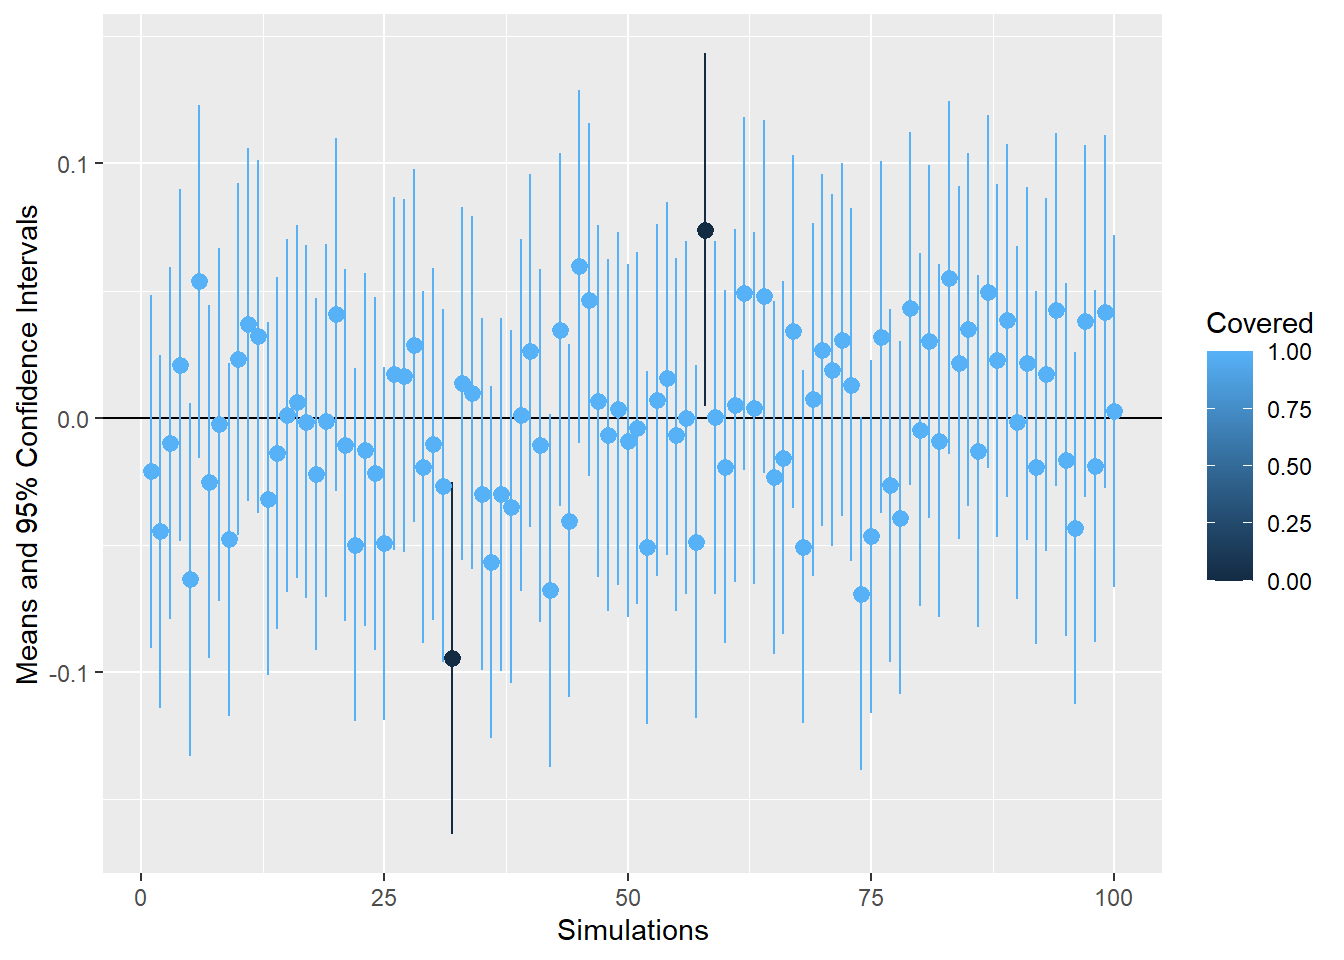
\includegraphics{gitbook-template-_files/figure-latex/unnamed-chunk-7-1.pdf}
In this case only two out of 100 CI's do not include the true population mean.

\hypertarget{the-central-limit-theorem}{%
\section{The Central Limit Theorem}\label{the-central-limit-theorem}}

Here we will also try to illustrate the \href{https://en.wikipedia.org/wiki/Central_limit_theorem}{Central Limit Theorem}, in it's most basic form, with a very simple example.

First we draw 1000 samples (again of size 800), form , say, a \emph{Poisson} distribution, of course we could've drawn them from a uniform or an exponential as well.

\begin{Shaded}
\begin{Highlighting}[]
\NormalTok{samples\_2 }\OtherTok{\textless{}{-}}\NormalTok{ samples }\OtherTok{\textless{}{-}}\NormalTok{plyr}\SpecialCharTok{::}\FunctionTok{rlply}\NormalTok{(}\DecValTok{1000}\NormalTok{, }\FunctionTok{rpois}\NormalTok{(}\DecValTok{800}\NormalTok{, }\DecValTok{2}\NormalTok{))}
\end{Highlighting}
\end{Shaded}

Now we calculate the mean for each sample:

\begin{Shaded}
\begin{Highlighting}[]
\NormalTok{means }\OtherTok{\textless{}{-}}\NormalTok{ samples\_2 }\SpecialCharTok{\%\textgreater{}\%}
  \FunctionTok{lapply}\NormalTok{(., mean) }\SpecialCharTok{\%\textgreater{}\%}
  \FunctionTok{as.data.frame}\NormalTok{() }\SpecialCharTok{\%\textgreater{}\%}
  \FunctionTok{t}\NormalTok{()}
\end{Highlighting}
\end{Shaded}

And now we plot a histogram of the resulting means:

\begin{Shaded}
\begin{Highlighting}[]
\FunctionTok{hist}\NormalTok{(}\FunctionTok{t}\NormalTok{(means))}
\end{Highlighting}
\end{Shaded}

\begin{figure}
\centering
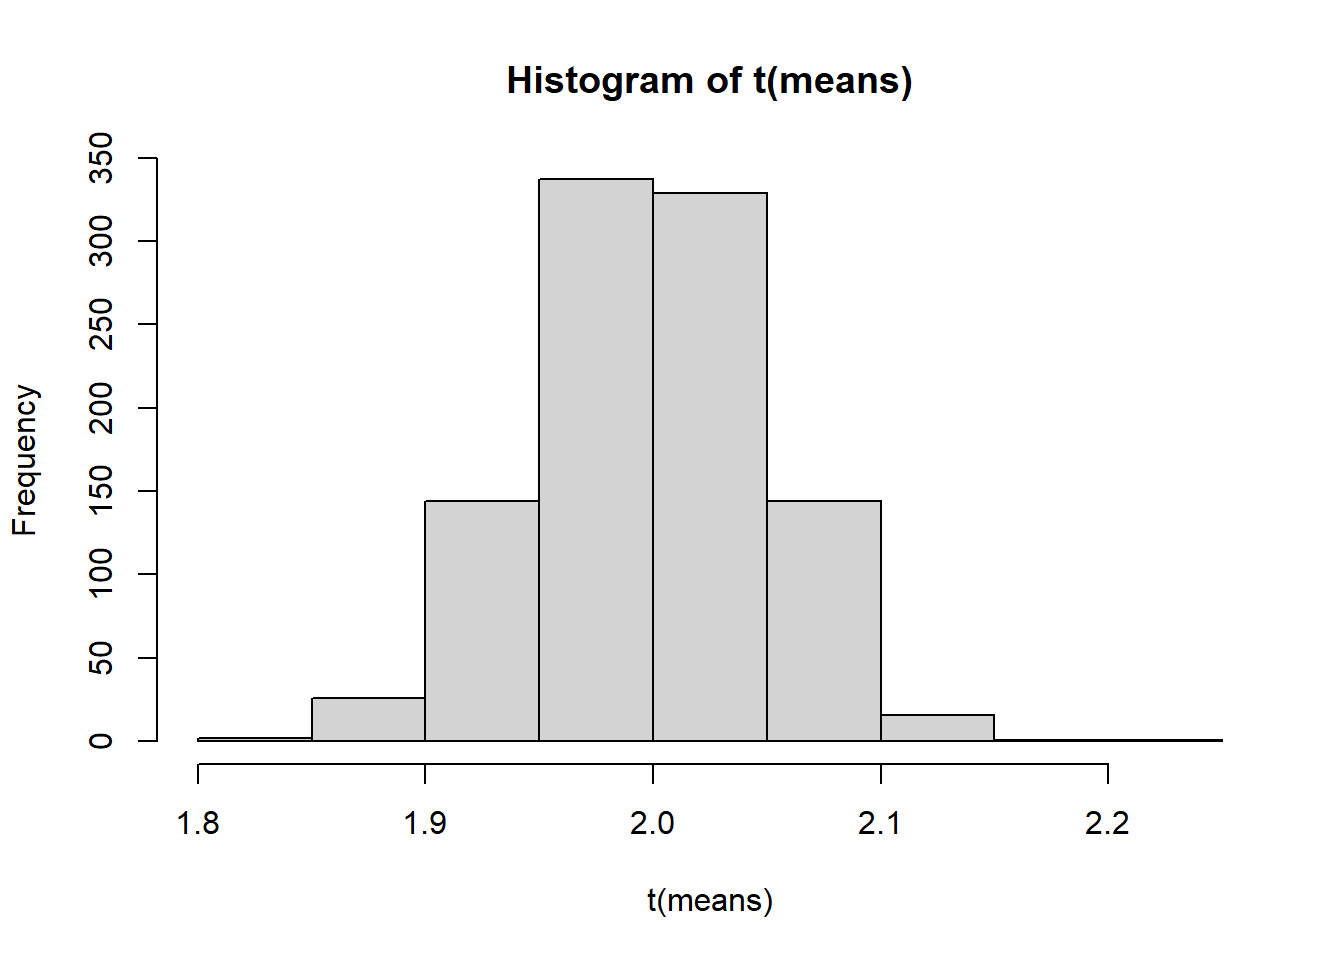
\includegraphics{gitbook-template-_files/figure-latex/unnamed-chunk-10-1.pdf}
\caption{\label{fig:unnamed-chunk-10}Histogram of the sampling distribution of the mean}
\end{figure}

\hypertarget{equations}{%
\chapter{Equations}\label{equations}}

\hypertarget{bayes-theorem}{%
\section{Bayes' theorem}\label{bayes-theorem}}

\begin{equation} 
p(\theta | D) = \frac{p(D|\theta) p(\theta)} {p(D)}
\label{eq:bayes}
\end{equation}

\hypertarget{normal-pdf}{%
\section{Normal PDF}\label{normal-pdf}}

\begin{equation} 
f(x) = \frac{1}{\sigma\sqrt{2\pi}}\exp\left(-\frac{1}{2}\left(\frac{x-\mu}{\sigma}\right)^{2}\right)
\label{eq:normal}
\end{equation}

This is how we refer to equations:
-see equation \eqref{eq:normal}

\hypertarget{literature}{%
\chapter*{Literature}\label{literature}}
\addcontentsline{toc}{chapter}{Literature}

\hypertarget{appendix-appendix}{%
\appendix}


\hypertarget{appendix-a}{%
\chapter*{Appendix A}\label{appendix-a}}
\addcontentsline{toc}{chapter}{Appendix A}

  \bibliography{book.bib,packages.bib}

\end{document}
